Los tiempos de ejecución y el uso de memoria se registraron en archivos CSV ubicados en \texttt{code/sorting/data/} \texttt{code/matrix\_multiplication/data/}. 

Las gráficas de los resultados se generan automáticamente con los scripts de Python definidos en el \texttt{Makefile}, ejecutando el objetivo \texttt{plots}, lo que permite reproducir las visualizaciones bajo cualquier infraestructura similar.

\subsection*{Resultados ordenamientos}

A continuación se muestran los resultados principales. Cada Gráfico comparara los cuatro algoritmos para un tipo de entrada, representando en el eje X el tamaño n y en el eje Y el tiempo medio de ejecución (ms)




\subsubsection*{Datos aleatorios}
Probando con datos aleatorios obtuvimos en promedio estos tiempos de ejecucion

\begin{table}[ht]
  \centering
  \begin{tabular}{lrrrr}

    Algoritmo  & SelectionSort\.(µs) & MergeSort\.(µs) & QuickSort\.(µs)  & \texttt{std::sort}\.(µs) \\

    10  & 0 & 0.002 & 0 & 0 \\
    1000& 2& 0.156& 0.053 & 0.066\\
    100000& 9498& 8.17&3.50&2.80\\
    10 000 000 & +$\infty$ & 987& 461 &364\\

  \end{tabular}
  \caption{Tiempos de ejecución promedio para datos aleatorios}
  \label{tab:sorting-results}
\end{table}


Como se aprecia en el cuadro~\ref{tab:sorting-results}, los tiempos de ejecución promedio para entradas ordenadas ascendente muestran una clara diferencia entre el comportamiento cuadrático de \texttt{SelectionSort} y las curvas $O(n\log n)$ de los demás algoritmos. Esta misma información se representa de forma visual en la Figura~\ref{fig:scatterplot_3}, donde la pendiente más pronunciada de la línea de \texttt{SelectionSort} contrasta con las trayectorias más suaves de \texttt{MergeSort}, \texttt{QuickSort} y \texttt{std::sort}.  

\begin{figure}[H]
    \centering
    \begin{minipage}[t]{0.5\textwidth}
        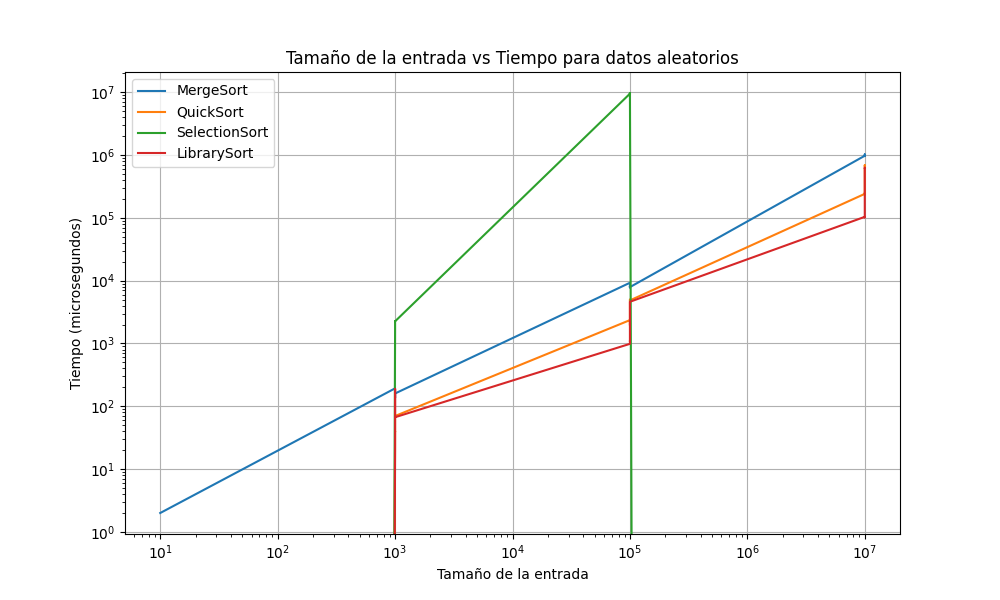
\includegraphics[width=\textwidth]{../code/sorting/data/plots/aleatorio_plot.png}
    \end{minipage}%
    \begin{minipage}[t]{0.5\textwidth}
        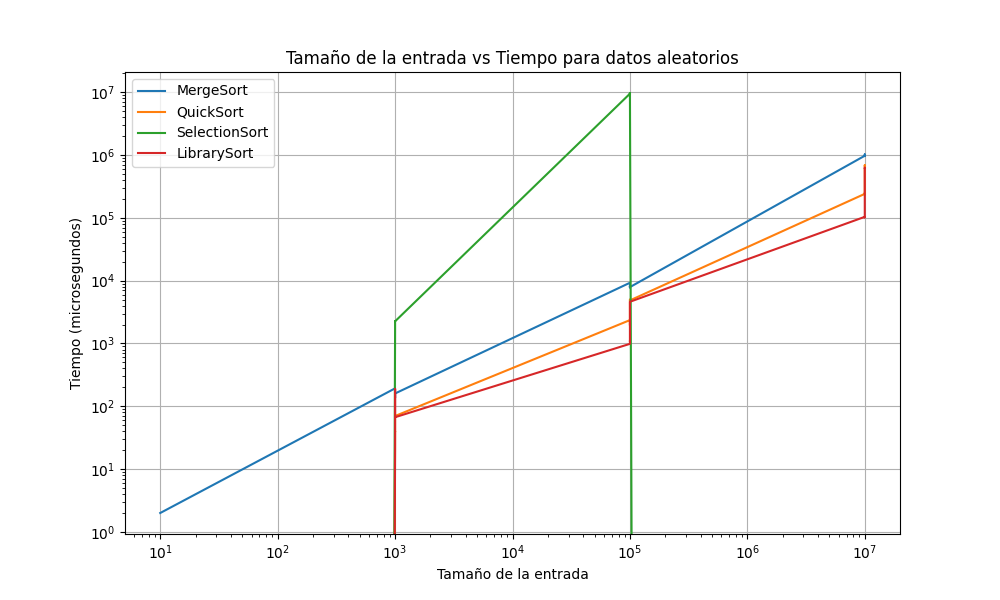
\includegraphics[width=\textwidth]{../code/sorting/data/plots/aleatorio_plot.png}
     \end{minipage}%
    \caption{Ejemplo de scatterplot hecho con matplotlib.}
    \label{fig:scatterplot_3}
\end{figure}

\subsubsection*{Datos ordenados de forma Ascendente}
Probando con datos ordenados de manera ascendente,  obtuvimos en promedio estos tiempos de ejecución

\begin{table}[ht]
  \centering
  \begin{tabular}{lrrrr}

    Algoritmo  & SelectionSort\.(µs) & MergeSort\.(µs) & QuickSort\.(µs)  & \texttt{std::sort}\.(µs) \\

    10  & 0 & 0.001 & 0 & 0 \\
    1000& 1.96& 0.105& 0.012 & 0.006\\
    100 000& 9432& 5.69&0.942&0.212\\
    10 000 000 & +$\infty$ & 722& 153 &18.04\\

  \end{tabular}
  \caption{Tiempos de ejecución promedio para datos ascendentes}
  \label{tab:sorting-results2}
\end{table}

Como se observa en la Tabla~\ref{tab:sorting-results2}, para entradas ordenadas ascendentemente los tiempos de \texttt{SelectionSort} igualmente  crecen de manera drástica en comparación con los algoritmos $O(n\log n)$.

Para $n=10$ los cuatro métodos tardan prácticamente $0\,\mathrm{ms}$, pero ya para $n=10^3$ \texttt{SelectionSort} registra $1.96\,\mathrm{ms}$ frente a $0.105\,\mathrm{ms}$ de \texttt{MergeSort}, $0.012\,\mathrm{ms}$ de \texttt{QuickSort} y $0.006\,\mathrm{ms}$ de \texttt{std::sort}. Al aumentar a $n=10^5$, \texttt{SelectionSort} alcanza $9432\,\mathrm{ms}$, mientras que \texttt{MergeSort}, \texttt{QuickSort} y \texttt{std::sort} se quedan en $5.69\,\mathrm{ms}$, $0.942\,\mathrm{ms}$ y $0.212\,\mathrm{ms}$, respectivamente. Para $n=10^7$, \texttt{SelectionSort} resulta inviable (+$\infty$), en contraste con los $722\,\mathrm{ms}$, $153\,\mathrm{ms}$ y $18.04\,\mathrm{ms}$ de \texttt{MergeSort}, \texttt{QuickSort} y \texttt{std::sort}.

Esta misma diferencia de escalado queda reflejada de manera más intuitiva en la Figura~\ref{fig:ordenadas_ascendente}, donde la curva de \texttt{SelectionSort} muestra una pendiente mucho más pronunciada en comparación con las trayectorias más planas de los algoritmos $O(n\log n)$. Así, la gráfica confirma visualmente la penalización  del comportamiento cuadrático de \texttt{SelectionSort} incluso en el “mejor caso” de entradas ya ordenadas.  

\begin{figure}[H]
    \centering
    \begin{minipage}[t]{0.5\textwidth}
        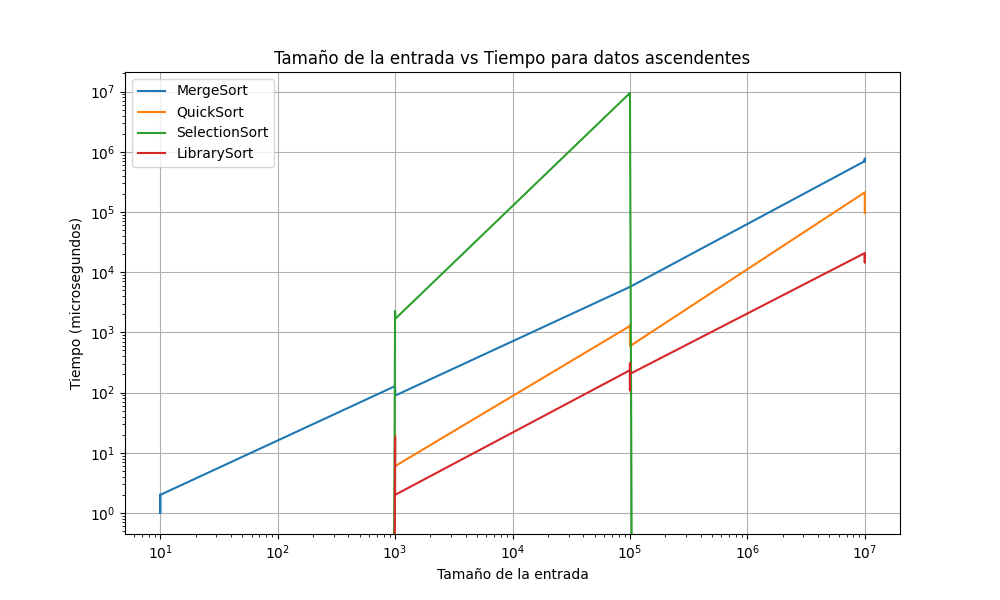
\includegraphics[width=\textwidth]{../code/sorting/data/plots/ascendente_plot.png}
    \end{minipage}%
    \begin{minipage}[t]{0.5\textwidth}
        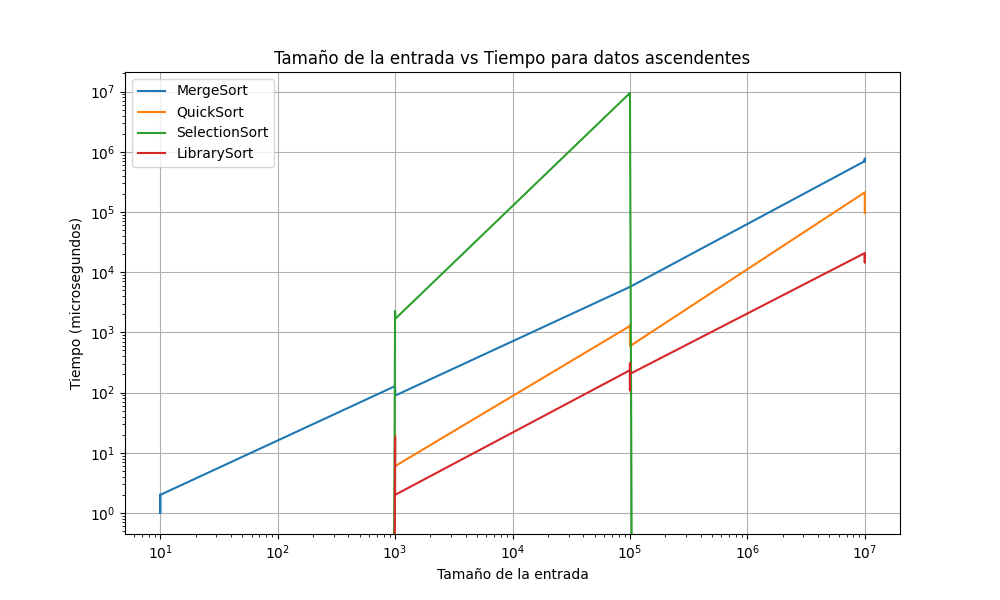
\includegraphics[width=\textwidth]{../code/sorting/data/plots/ascendente_plot.png}
     \end{minipage}%
    \caption{Ejemplo de scatterplot hecho con matplotlib.}
    \label{fig:ordenadas_ascendente}
\end{figure}

\newpage

\subsubsection*{Datos ordenados de forma descendente}

Probando con datos ordenados de manera descendente,obtuvimos en promedio estos tiempos de ejecución


\begin{table}[ht]
  \centering
  \begin{tabular}{lrrrr}

    Algoritmo  & SelectionSort\.(µs) & MergeSort\.(µs) & QuickSort\.(µs)  & \texttt{std::sort}\.(µs) \\

    10  & 0 & 0.001 & 0.0001 & 0 \\
    1000&1.62&  0.091& 0.009 & 0.008\\
    100 000& 9422& 5.81&0.924&0.188 \\
    10 000 000 & +$\infty$ &  746& 142 &18.66\\

  \end{tabular}
  \caption{Tiempos de ejecución promedio para datos descendentes}
  \label{tab:sorting-results3}
\end{table}

Como se aprecia en la Tabla~\ref{tab:sorting-results3}, cuando los datos llegan ya ordenados de forma descendente, el rendimiento de \texttt{SelectionSort} se ve gravemente afectado, hasta el punto de volverse inviable para tamaños muy grandes. En contraste, \texttt{MergeSort}, \texttt{QuickSort} y \texttt{std::sort} conservan su comportamiento $O(n\log n)$, sufriendo únicamente un incremento moderado en los tiempos de ejecución. Esta disparidad en la escalada de tiempos queda de manifiesto en la Figura~\ref{fig:sorting-descendente}, donde las curvas de los algoritmos que usan dividir y conquistar muestran pendientes suaves frente a la pronunciada pendiente observada en \texttt{SelectionSort}.  

\begin{figure}[H]
    \centering
    \begin{minipage}[t]{0.5\textwidth}
        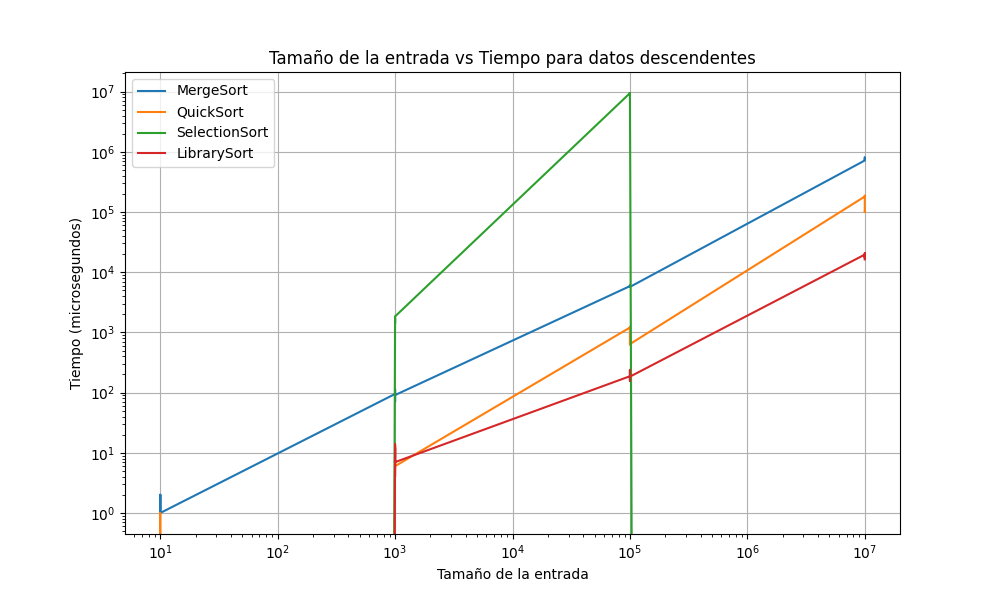
\includegraphics[width=\textwidth]{../code/sorting/data/plots/descendente_plot.png}
    \end{minipage}%
    \begin{minipage}[t]{0.5\textwidth}
        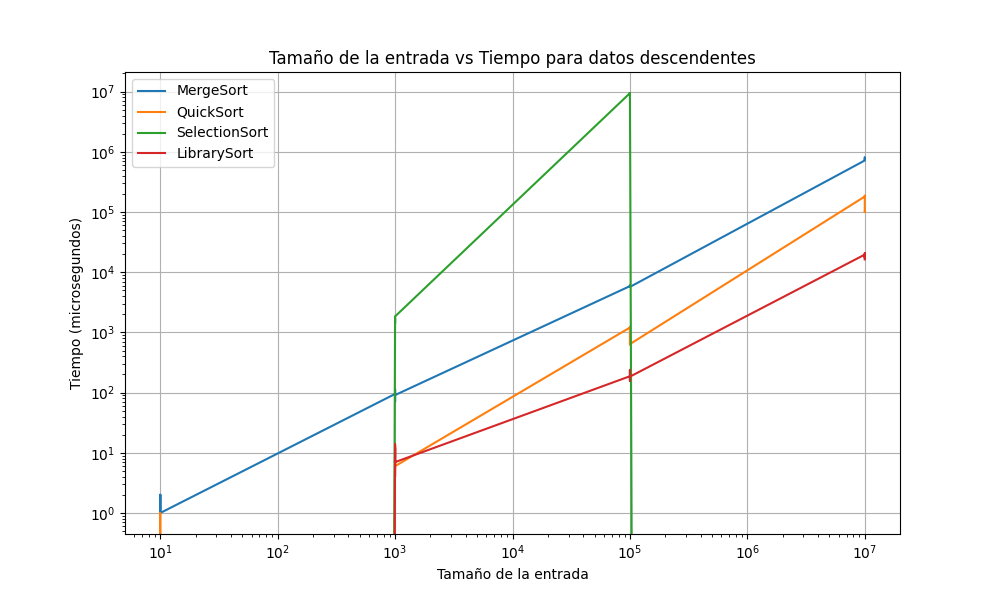
\includegraphics[width=\textwidth]{../code/sorting/data/plots/descendente_plot.png}
     \end{minipage}%
    \caption{Ejemplo de scatterplot hecho con matplotlib.}
    \label{fig:sorting-descendente}
\end{figure}


\newpage

\subsection*{Resultados Multiplicación de Matrices}

A continuación se presentan los resultados principales de los dos algoritmos de multiplicación de matrices implementados. Cada gráfico compara dichos algoritmos para un tipo de entrada distinto, representando en el eje X el tamaño de la matriz $n$ considerando matrices cuadradas de dimensión ($n \times n$) y en el eje Y el tiempo medio de ejecución (en milisegundos).

A continuación se muestran los gráficos detallados para cada tipo de entrada y un breve análisis de sus implicaciones prácticas.

\subsubsection*{Matrices Densas}

Probando con matrices densas  se obtuvieron en prodmedio los siguientes tiempos de ejecucion

\begin{table}[ht]
  \centering
  \begin{tabular}{lrr}

    Tamanño ($n \times n$)  & Naive\.(ms) & Strassen\.(ms)\\

    16  & 0.132 & 0.345  \\
    64  & 2.63  & 2.88\\
    256& 102& 98\\
    1024& 6459 &  6650\\

  \end{tabular}
  \caption{Tiempos de ejecución promedio para matrices densas}
  \label{tab:sorting-results4}
\end{table}

La Tabla \ref{tab:sorting-results4} muestra los tiempos promedio de ejecución obtenidos para la multiplicación de matrices densas utilizando los algoritmos Naive y Strassen. Se observa que, para tamaños pequeños, ambos algoritmos presentan tiempos similares, aunque Strassen resulta ligeramente más lento en =
n=16 debido al mayor overhead de su estructura recursiva. Sin embargo, a medida que el tamaño de las matrices crece, las diferencias se atenúan e incluso Strassen logra superar marginalmente al método Naive en n=256. en la figura \ref{fig:multi_densa} Para tamaños mayores,como n=1024, ambos algoritmos exhiben tiempos de ejecución similares, lo que sugiere que el impacto teórico de Strassen en la reducción de complejidad se ve amortiguado por factores prácticos como el manejo de memoria y la sobrecarga de recursión.

\begin{figure}[H]
    \centering
    \begin{minipage}[t]{0.5\textwidth}
        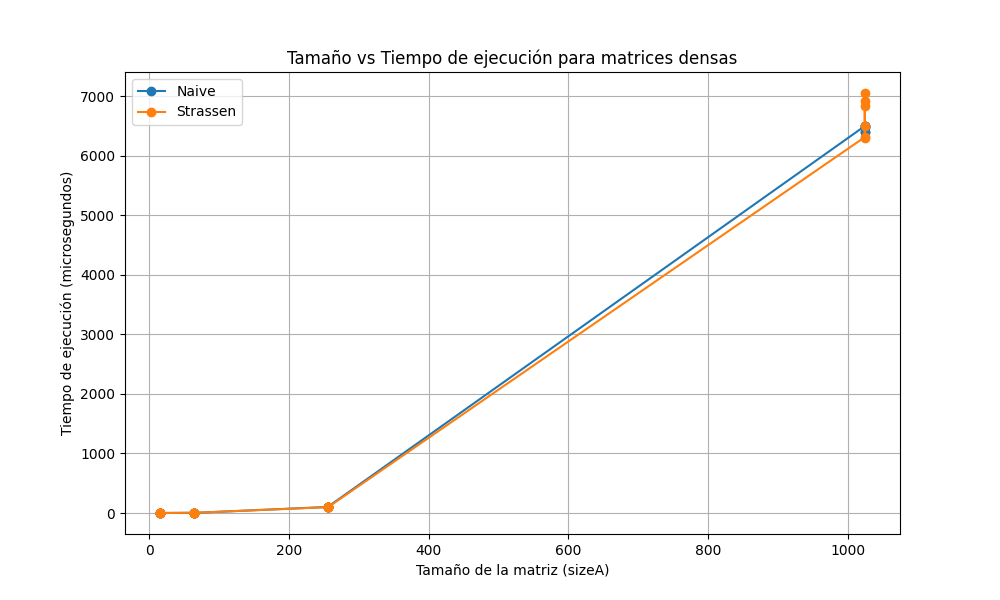
\includegraphics[width=\textwidth]{../code/matrix_multiplication/data/plots/dense_matrices_plot.png}
    \end{minipage}%
    \begin{minipage}[t]{0.5\textwidth}
        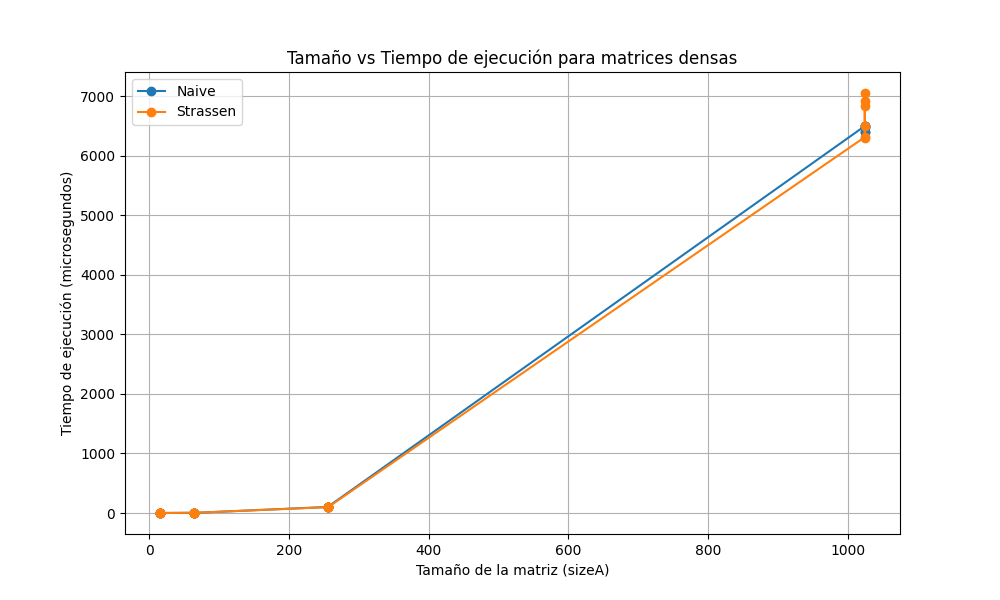
\includegraphics[width=\textwidth]{../code/matrix_multiplication/data/plots/dense_matrices_plot.png}
     \end{minipage}%
    \caption{Ejemplo de scatterplot hecho con matplotlib.}
    \label{fig:multi_densa}
\end{figure}

\subsubsection*{Matrices Diagonales}

Probando con Matrices Diagonales  se obtuvieron en prodmedio los siguientes tiempos de ejecución

\begin{table}[ht]
  \centering
  \begin{tabular}{lrr}

    Tamanño ($n \times n$)  & Naive\.(ms) & Strassen\.(ms)\\

    16  & 0.065 & 0.161  \\
    64  & 1.59  & 1.86\\
    256& 102& 96.71\\
    1024& 6498 &  6623\\

  \end{tabular}
  \caption{Tiempos de ejecución promedio para matrices diagonales}
  \label{tab:sorting-results5}
\end{table}

La Tabla \ref{tab:sorting-results5} recoge los tiempos promedio de ejecución para multiplicación de matrices diagonales, y el Gráfico \ref{fig:multi_diagonal} ilustra de forma visual esta evolución. Al comparar estos resultados con los obtenidos previamente para matrices densas, se aprecia que ambos algoritmos (Naive y Strassen) obtienen un marcado beneficio en el caso diagonal: los tiempos iniciales para \(n=16\) y \(n=64\) se reducen casi a la mitad respecto al escenario denso, reflejando la simplicidad del cómputo sobre estructuras con elementos mayoritariamente nulos. No obstante, para tamaños grandes (\(n=256\) y \(n=1024\)) las diferencias se atenúan, y los tiempos convergen nuevamente a valores similares, puesto que la sobrecarga de recorrido y acceso a memoria acaba dominando el coste total. Este contraste evidencia cómo la naturaleza de la matriz influye en el rendimiento de los algoritmos y subraya la importancia de seleccionar métodos adaptados al patrón de datos.

\begin{figure}[H]
    \centering
    \begin{minipage}[t]{0.5\textwidth}
        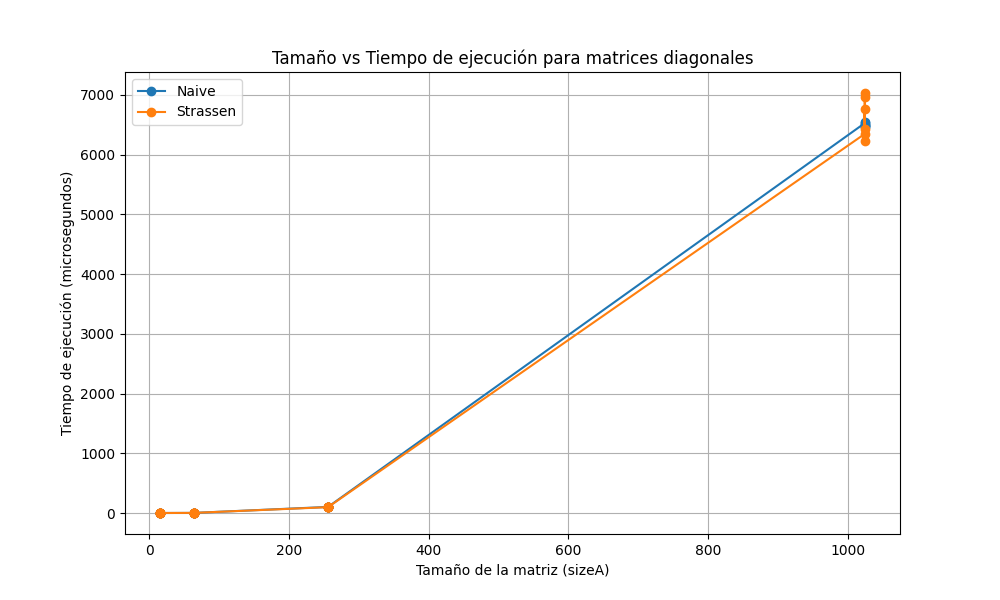
\includegraphics[width=\textwidth]{../code/matrix_multiplication/data/plots/diagonal_matrices_plot.png}
    \end{minipage}%
    \begin{minipage}[t]{0.5\textwidth}
        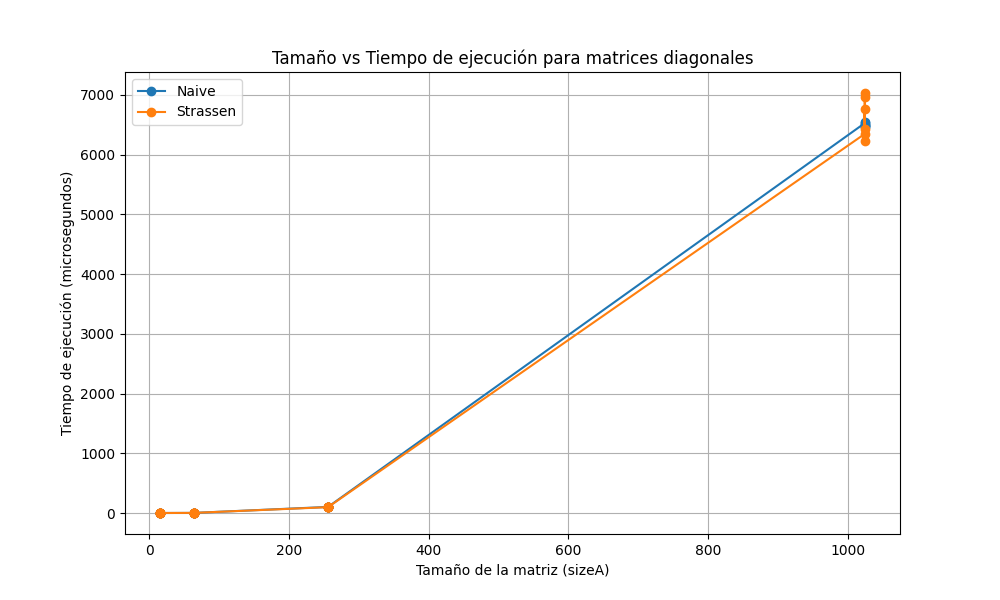
\includegraphics[width=\textwidth]{../code/matrix_multiplication/data/plots/diagonal_matrices_plot.png}
     \end{minipage}%
    \caption{Ejemplo de scatterplot hecho con matplotlib.}
    \label{fig:multi_diagonal}
\end{figure}

\newpage
\subsubsection*{Matrices Dispersa}

Probando con Matrices Dispersas  se obtuvieron en promedio los siguientes tiempos de ejecución

\begin{table}[ht]
  \centering
  \begin{tabular}{lrr}

    Tamanño ($n \times n$)  & Naive\.(ms) & Strassen\.(ms)\\

    16  & 0.055 & 0.144  \\
    64  & 1.561  & 1.782\\
    256& 104& 113\\
    1024& 6555 &  6819\\

  \end{tabular}
  \caption{Tiempos de ejecución promedio para matrices dispersas}
  \label{tab:dispersa-result}
\end{table}

La Tabla \ref{tab:dispersa-result} presenta los tiempos promedio de ejecución para la multiplicación de matrices dispersas, mientras que el Gráfico \ref{fig:multi_dispersa} ilustra la evolución de estos valores en función del tamaño \(n\). En comparación con los resultados de matrices densas y diagonales, observamos que para tamaños reducidos (\(n=16\) y \(n=64\)) los algoritmos Naive y Strassen se benefician de la escasez de elementos no nulos, mostrando tiempos incluso inferiores a los de las matrices diagonales, y muy por debajo de los obtenidos en el escenario denso. Sin embargo, al aumentar \(n\) (especialmente a partir de \(256\)), las mejoras se diluyen: el método Naive alcanza valores de tiempo similares (e incluso ligeramente superiores) a los de matrices densas, y Strassen incurre en un costo extra por la gestión de la estructura dispersa, superando en algunos casos los tiempos registrados para matrices diagonales. Este comportamiento pone de manifiesto que, aunque la dispersidad aporta ventajas en cómputos pequeños, el sobrecoste de recorrer y verificar la ubicación de los ceros puede contrarrestar la ganancia teórica en instancias de gran tamaño.

\begin{figure}[H]
    \centering
    \begin{minipage}[t]{0.5\textwidth}
        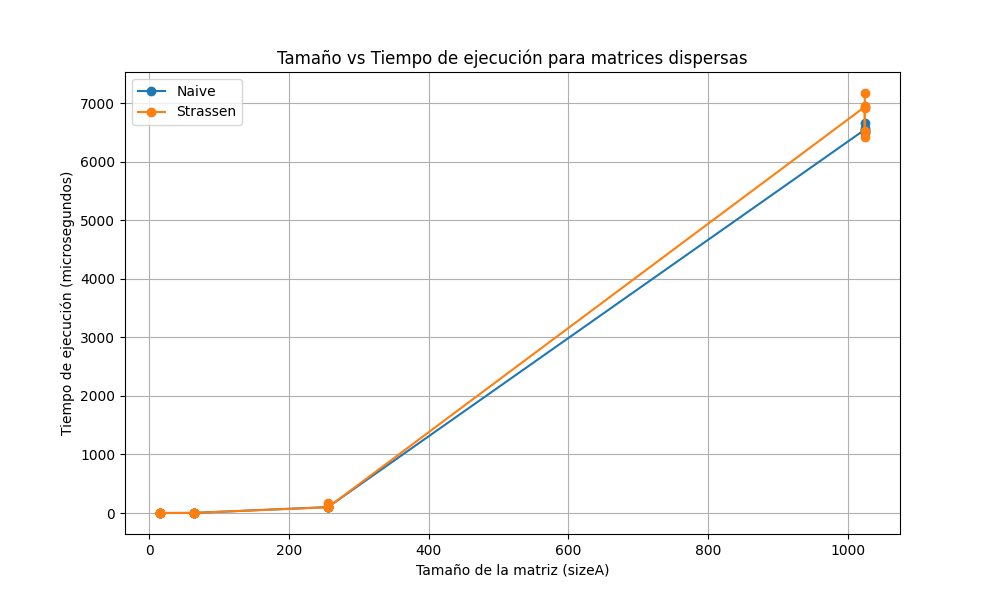
\includegraphics[width=\textwidth]{../code/matrix_multiplication/data/plots/sparse_matrices_plot.png}
    \end{minipage}%
    \begin{minipage}[t]{0.5\textwidth}
        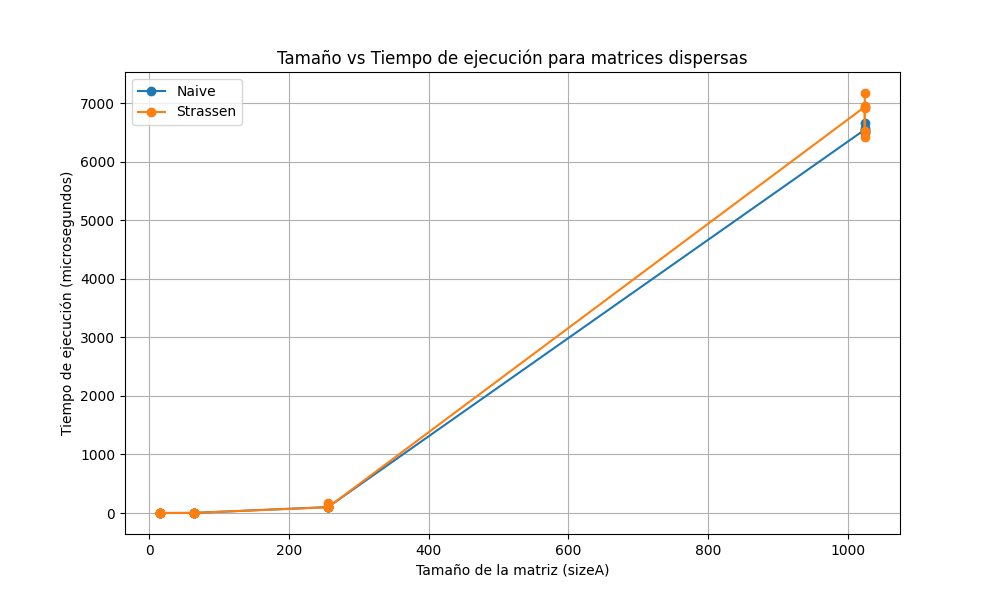
\includegraphics[width=\textwidth]{../code/matrix_multiplication/data/plots/sparse_matrices_plot.png}
     \end{minipage}%
    \caption{Tiempos de ejecución promedio para matrices dispersas}
    \label{fig:multi_dispersa}
\end{figure}